\documentclass[a4paper,10pt]{article}
\usepackage{graphicx}
\usepackage[dutch]{babel}

\title{Software Engineering en Gedistribueerde Applicaties \\[10pt]Werkplan\\[25pt]Team F.A.C.H.T.}
\author{\\Chris Bovenschen, Harm Dermois, \\Alexandra Moraga Pizarro, Tamara Ockhuijsen en Fredo Tan \\[10pt]6104096, 0527963, 6129544, 6060374 , 6132421 \\[25pt]Universiteit van Amsterdam}
\begin{document}
\maketitle

\newpage
\tableofcontents

\newpage
\section{Inleiding}
Dit is het werkplan van team F.A.C.H.T. voor het vak Software Engineering en Gedistribueerde
Applicaties. In dit document zijn de planning, de deliverables, de modules en het model te vinden van ons project. De voorzitter is Harm Dermois. De secretarissen zijn ingedeeld als volgt:
\begin{itemize}
\item Week 1: Fredo Tan
\item Week 2: Alexandra Moraga Pizarro
\item Week 3: Tamara Ockhuijsen
\item Week 4: Chris Bovenschen
\end{itemize}
Het doel is een robot te maken die zelf rond kan rijden en een map kan maken. Nadat er een map is gemaakt, kan de robot een pad plannen die je van punt A naar B brengt.
\section{Model}
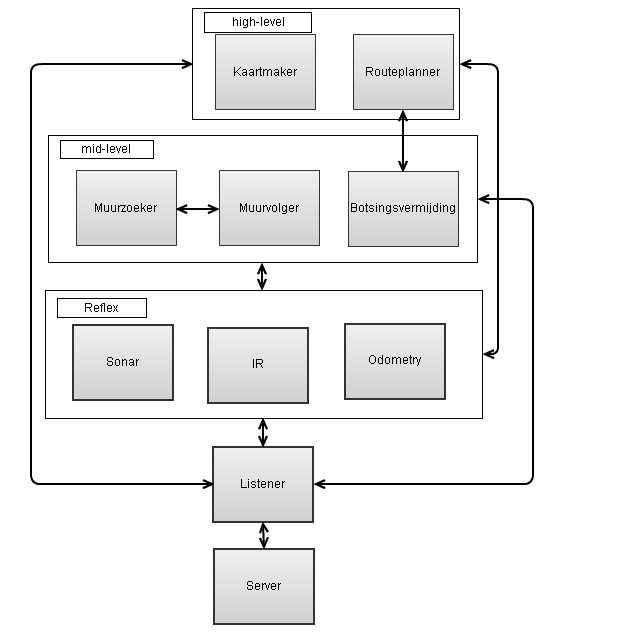
\includegraphics[scale = 0.5]{flowchart.PNG}\\\\
Alle grijze blokken zijn modules.\\
\newpage
De listenermodule is verbonden aan de server via een TCP-verbinding. Deze wordt tevens gebruikt om commando's naar de robot te sturen. De ontvangen sensor data wordt doorgegeven naar de sensormodules, die kijken of de data daadwerkelijk geldig is en binnen de parameters valt, zodat we de data van de robot kunnen gebruiken. We hebben drie sensormodules waar we informatie vandaan halen: sonar, laser en odometry. Vanuit deze laag gaat de data naar de laag waar de mid-level modules zich bevinden, die dienen voor de muurzoeker en muurvolger. De data voor de kaartenmakermodule komt rechtstreeks uit de sensormodules. Berekende kaarten uit de kaartenmaker kunnen gebruikt worden voor de routeplanner. De routeplanner geeft zijn berekende pad tenslotte door aan de movementsmodule. De botsingvermijder is een module die botsingen kan detecteren en aan de andere modules meldt wanneer er een botsing zal gaan plaatsvinden.
We hebben gekozen voor dit model om het wat robuuster te maken. Als de listener het niet doet, werkt het hele programma niet, maar als er \'{e}\'{e}n van de sensormodules is uitgevallen, kan het programma
nog steeds blijven draaien. Ook hebben we het gedrag van de robot dus opgedeeld in drie verschillende modules, namelijk: muurzoeker, muurvolger en routeplanner. Van deze modules kan er maar 1 tegelijk aanstaan. 

\section{Deliverables}
Aan het eind van het project leveren we een robot die zich kan voortbewegen door middel van berekeningen die gebaseerd zijn op data afkomstig van de sensoren. Vervolgens is het de bedoeling dat de robot diens omgeving in kaart kan brengen met behulp van de informatie van de sensoren. De robot moet in staat zijn om in een vrij volle ruimte gevuld met diverse obstakels een pad langs een wand te kunnen afleggen.
Dus wij leveren de volgende modules:
\begin{enumerate}
\item De movements.
\item Een listener.
\item Reflex/sensormodules per soort data.
\item Een muurzoeker.
\item Een muurvolger.
\item Een botsingvermijder.
\item Een routeplanner.
\item Een mapmaker.
\item Een communicator die tussen modules kan praten.
\item Een werkend geheel die alle modules met elkaar combineert.
\end{enumerate}
Uitleg over de modules is te vinden in sectie \ref{sec:modules}.
Bij de eerste deliverable leveren we de volgende modules: De listener, muurvolger, muurzoeker, reflex/sensor en communicator. Deze staan allemaal op zichzelf en maken hun eigen verbinding met de server. De tweede deliverable is het eindproduct en dan hebben we een werkend geheel.
\section{Testen}
Alle modules gaan we apart testen. We gaan elke module direct aan de simulator vast zetten en met de directe data de modules testen. Wanneer de modules werken, gaan we ze verder testen op onconventionele omstandigheden. De pre-condities worden aan het begin van de methode gedefinieerd. Wanneer er in de module waardes aankomen die niet voldoen aan de pre-condities, worden die genegeerd. Al deze modules worden later gemodificeerd met de communicator methode, zodat ze met elkaar kunnen praten.

\section{Modules}
\label{sec:modules}
Alle modules worden voorzien van een communicator. Deze communicator leest uit waar alle modules zich bevinden. Wanneer de communicator wordt opgestart, wordt er een thread aangemaakt die verbindingen kan aannemen. Deze thread start op zijn beurt nog een andere thread op die luistert naar alle inkomende requests en handelt deze af. Het precieze protocol voor de communicatie moet nog nader worden bepaald. \\
Onze definitie van een muur omvat alle obstakels die we zien. Wij gebruiken geen camera, dus het is niet mogelijk om het verschil te zien tussen een muur en een blok die in de weg staat.\\

\subsection{Movements}
Dit is een bibliotheek waar alle bewegingen in zijn gedefinieerd. Deze kan ge\"{i}mporteerd worden door alle modules die de robot willen veranderen.
\subsection{Listener}
De listener is de module die direct aan de server vast zit. Deze haalt de informatie binnen die de robot opstuurt, maar stuurt ook commando's naar de robot. Dit maakt de commando's naar de robot in ieder geval consistent. De data die wordt ontvangen, wordt direct opgestuurd naar de respectievelijke reflexmodules die de data dan verder bewerken. Het is mogelijk om levels toe te voegen voor de urgentie van de commando's.
\subsection{Reflexmodules}
De reflexmodules krijgen de respectievelijke data van de listener. Deze modules zijn een soort opslagplaats voor de meest recente data die de listener heeft gekregen. Deze modules kunnen de robot ook stoppen wanneer de data die ze binnen krijgen niet binnen de verwachte parameters vallen. Deze modules kunnen door de high-level modules aangeroepen worden voor de meest recente data.
\subsection{Botsingvermijder}
De botsingvermijder hoort bij de routeplannermodule. Deze methode runt alleen wanneer de routeplanner aan het werken is. Deze detecteert dingen die zich niet op de map bevinden. De botsingvermijder wordt dus alleen gebruikt voor dingen die onvoorzien zijn.
\subsection{Muurzoeker}
De muurzoeker is de mode voor de robot wanneer hij de wereld moet verkennen. De robot begint om zich heen te kijken, de kleinste waarde op te zoeken en zich daarheen te bewegen. Wanneer er een bepaalde drempelwaarde is bereikt, gaan we ervan uit dat er een muur is gevonden en gaan we over naar de muurvolgermodule die dan verder gaat met de gevonden muur te volgen.
\subsection{Muurvolger}
De muurvolger volgt de muur die door de muurzoeker gevonden is. Bij de gevonden muur draait de robot 90 graden, zodat de kleinste waarde van de sonar in de meest rechtersensor te vinden is. Hierna blijft hij rechtdoor rijden totdat er geen muur meer is om te volgen en gaat dan weer over naar de muurzoeker.
\subsection{Routeplanner}
De routeplanner kan alleen gebruikt worden wanneer er al een map is gemaakt en kan dus alleen een route plannen binnen een bekend domein. Hierin probeert hij een zo kort mogelijk pad te vinden naar de bestemming. 
\subsection{Mapmaker}
De mapmaker krijgt een constante stroom van sonar, IR en odometry data waarmee hij een map gaat maken.
\section{Planning}
Er zijn vier weken beschikbaar voor dit project. In de eerste week van het project wordt de listener als eerst gerealiseerd. Daarnaast wordt de module die de methoden bevat voor de bewegingen geschreven. Wanneer die is geschreven, maken we in dezelfde week nog een begin aan de sensormodules. De drie modules muurzoeker, muurvolger en botsingsvermijder zijn de volgende componenten die ge\"{i}mplementeerd moeten worden. Dat willen we graag in de tweede week doen. Wanneer dat voltooid is, maken we de high-level componenten aan: de routeplanner en de kaartenmaker. We denken dat deze twee onderdelen vrij gecompliceerd zijn, hier willen we dan ruim de tijd voor nemen.\\

17 juni is de dag wanneer de eerste deliverable gereed moet zijn. De eerste deliverable omvat de listener, bewegingen en (een deel van) de mid-level componenten. In de derde week vindt het inleveren van de tweede deliverable plaats. Op 23 juni hebben we de mid-level componenten en de high-level componenten gereed.\\
Onze focus en deliverables per week:\\
\begin{tabular}{|l|p{5cm}|p{5cm}|}
\hline
Week&Focus&Deliverables\\
\hline
week 1&listener, movements, sensoren en schets werkplan& listener, movements, sensoren en schets werkplan \\ 
\hline
week 2&definitieve werkplan, mid-level modules en tests& werkplan en mid-level modules\\
\hline
week 3&mapmaker, routeplanner en tests & mapmaker\\
\hline
week 4& eindverslag, opschonen code en testen& eindcode en verslag\\
\hline

\end{tabular}

\end{document}
